\documentclass[11pt]{article}
\usepackage[paperwidth=30cm,paperheight=30cm,margin=5mm]{geometry}
\usepackage[T1]{fontenc}
\usepackage{tikz}
\usetikzlibrary{arrows.meta,positioning,fit,backgrounds,calc,shapes.geometric}
\pagestyle{empty}
\tikzset{
  box/.style={draw, rounded corners=2pt, align=center, font=\small, minimum height=9mm, inner sep=4pt, fill=white},
  data/.style={box, fill=blue!8},
  model/.style={box, fill=orange!12},
  outp/.style={box, fill=green!10},
  frozen/.style={box, dashed, font=\small\itshape},
  arr/.style={-{Latex[length=2mm]}, semithick},
  lbl/.style={font=\scriptsize, align=center},
  group/.style={draw, rounded corners=4pt, dashed, gray, inner sep=6pt},
  glbl/.style={font=\scriptsize\itshape, gray, anchor=south west, inner sep=1pt}}
\begin{document}

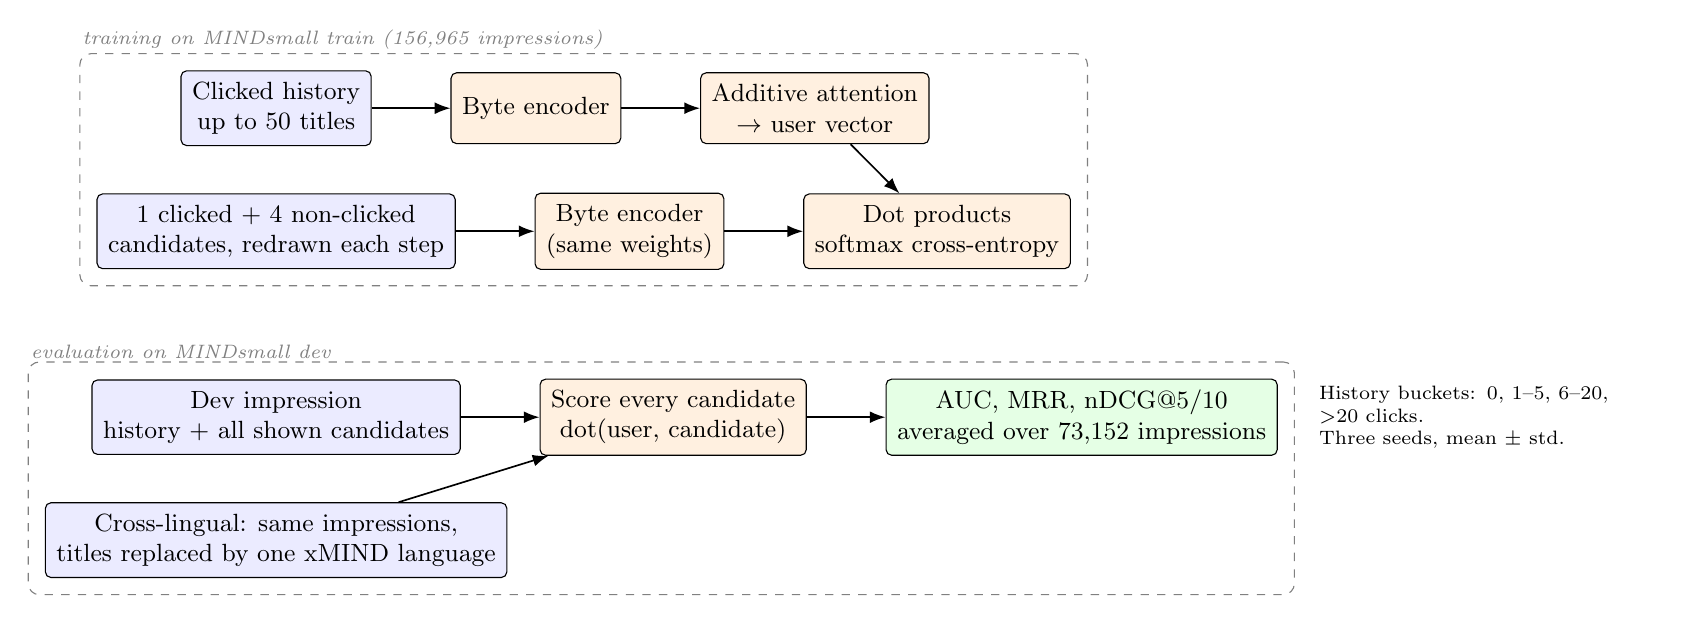
\begin{tikzpicture}[node distance=6mm and 10mm]
  % training
  \node[data] (hist) {Clicked history\\up to 50 titles};
  \node[model, right=of hist] (enc1) {Byte encoder};
  \node[model, right=of enc1] (user) {Additive attention\\$\to$ user vector};
  \node[data, below=of hist] (cand) {1 clicked + 4 non-clicked\\candidates, redrawn each step};
  \node[model, right=of cand] (enc2) {Byte encoder\\(same weights)};
  \node[model, right=of enc2] (dot) {Dot products\\softmax cross-entropy};
  \draw[arr] (hist) -- (enc1); \draw[arr] (enc1) -- (user); \draw[arr] (cand) -- (enc2); \draw[arr] (enc2) -- (dot);
  \draw[arr] (user) -- (dot);
  % evaluation
  \node[data, below=14mm of cand] (imp) {Dev impression\\history + all shown candidates};
  \node[model, right=of imp] (score) {Score every candidate\\dot(user, candidate)};
  \node[outp, right=of score] (metrics) {AUC, MRR, nDCG@5/10\\averaged over 73,152 impressions};
  \draw[arr] (imp) -- (score); \draw[arr] (score) -- (metrics);
  \node[data, below=of imp] (swap) {Cross-lingual: same impressions,\\titles replaced by one xMIND language};
  \draw[arr] (swap) -- (score);
  \node[lbl, right=4mm of metrics, text width=4.2cm, align=left] {History buckets: 0, 1--5, 6--20, $>$20 clicks.\\Three seeds, mean $\pm$ std.};
  \begin{scope}[on background layer]
    \node[group, fit=(hist)(user)(cand)(dot), label={[glbl]north west:training on MINDsmall train (156,965 impressions)}] {};
    \node[group, fit=(imp)(metrics)(swap), label={[glbl]north west:evaluation on MINDsmall dev}] {};
  \end{scope}
\end{tikzpicture}
\end{document}
